%\setlength{\belowcaptionskip}{-15pt}
%\setlength{\abovecaptionskip}{0pt}
\section{Model and discretization}~\label{sec:model_disc}

In this section, the heat equation for the bolometer and a model for the
readout circuit are described.

\subsection{Heat equation for the bolometer}

The resistance $R(T)$ of the bolometer is a function of the
temperature $T$, which for
metals and semiconductors can be described by~\cite{xiu2010research}
\begin{equation}
  \label{eq:resistance_temperature}
  R(T)=R_s e^{\alpha(T-T_s)},
\end{equation}
where $\alpha$ is a constant that depends on the material of the
bolometer, and $R_s$ is the resistance of the bolometer at the
substrate temperature $T_s$.

The temperature of the bolometer as a function of time (and the
incoming IR radiation) can be described by the heat equation, the
Stefan-Boltzmann law and the Joule heating law
\begin{align} \label{eq:heat_balance_equation}
 C\frac{dT}{dt}&=\frac{V_b(t)^2}{R(T)}+\varepsilon(P_t+P_s -2A_s \sigma T^4)-G_{leg}(T-T_s), \\
 T(0)&=T_s.	\nonumber
\end{align}
Here $V_b(t)$ is the input voltage, $\varepsilon_e$ is the material
specific emissivity of the bolometer, $P_t$ is the radiation power from
the scene, $P_s$ is the radiation power from the substrate, $2A_s$ is
the total surface area of the bolometer (upside and downside), $\sigma$ is
the Boltzmann constant, and $G$
is thermal conductivity of the supporting legs. The term
$V_b(t)^2/R(T)$ is the power resulting from Joule heating, that is
the power induced by the bias voltage over
the bolometer, and $2A_s \sigma T^4$ represents the radiation power
emitted from the bolometer according to Stefan-Boltzmann's law. The
latter also relates $P_t$ to the target temperature $T_t$ of a scene
object as $P_t \propto T_t^4$.



\subsection{Readout voltage equation}

Each pixel of an IR camera can be modeled as the circuit in Figure~\ref{fig:circuit}.
\begin{figure}[ht]
 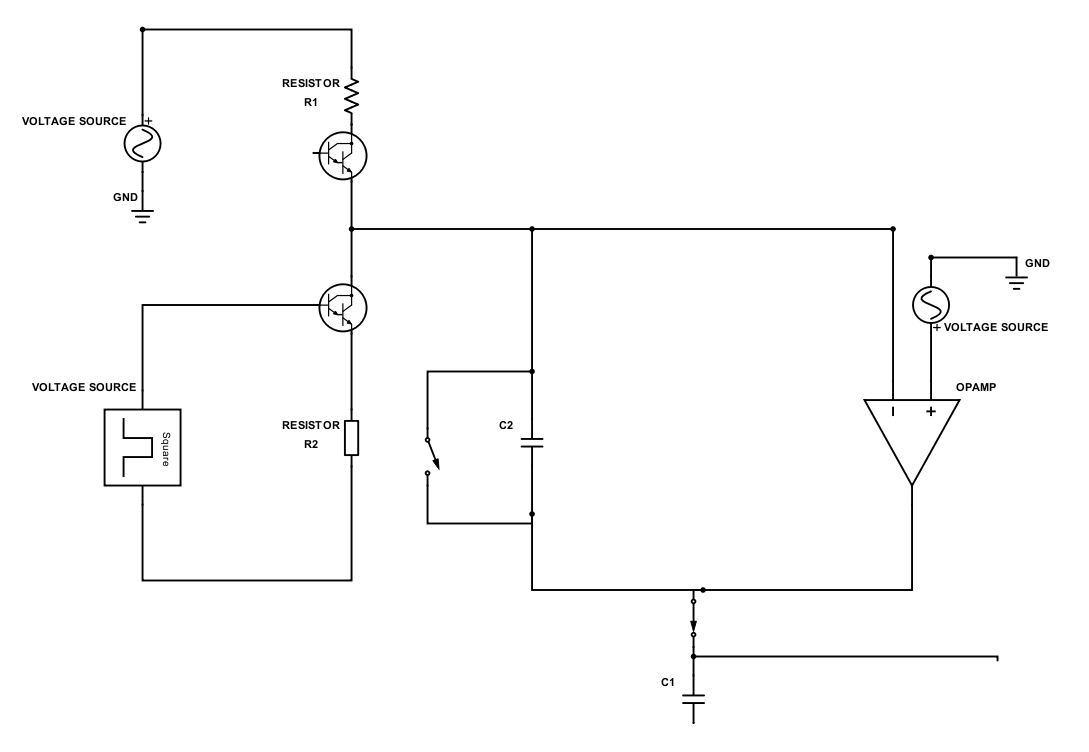
\includegraphics[scale=0.31]{gfx/circuit.png}
\caption{Circuit schematic that model a pixel of the IR camera generated with \url{https://www.digikey.com/schemeit}.}
\label{fig:circuit}
\end{figure}
More precisely the resistance of the bolometer corresponds to the resistor
R2. To measure the resistance $R(T)$ a bias voltage is applied over the resistance R2. The bias voltage, however, excessively heats up the
bolometer, and consequently the bias voltage is periodically shut off
to let the bolometer cool down. This results in an input signal for the bias
voltage that is a periodic square signal
\begin{align} \label{eq:Vb}
 V_b(t)&=\begin{cases} v_b & n t_f < t < n t_f + t_i \\
 0 &\mbox{ otherwise.}
 \end{cases} && n \in {\mathbb N}
\end{align}
The resulting current from R2, is then subtracted from the current
yielded from the resistance R1. This difference in current is then
fed to the capacitor C2, which functions as an integrator. The voltage
over the capacitor C2 is the readout voltage
$V_{samp}$. Using Kirchhoff's law, this voltage is expressed as
\begin{align} \label{eq:Vsamp_def}
 V_{samp} =
 \frac{1}{\tilde C} \int_{n t_f}^{n t_f + t_i} \left( \frac{V_0}{R_S} - \frac{V_b(s)}{R(T(s))} \right) ds + E
\end{align}
where $\tilde C$ is
the capacitance of C2. Clearly, in order to compute this integral, we
need to know the temperature as function of the time. This relation is
described by~\eqref{eq:heat_balance_equation}. Notice that $V_{samp}$
does not depend on $R(T)$ if $V_b = 0$, and thus it is only relevant to
integrate up to time $t_i$.

The output signal can therefore be simulated in the following way. We
set an initial temperature $T_0$ for the bolometer and solve the heat
balance equation~\eqref{eq:heat_balance_equation}. Then we compute the
integral describing the readout signal~\eqref{eq:Vsamp_def}.


\subsection{Illustrative example}~\label{sec:example}

A reasonable and realistic simulation of the bolometer response can be
obtained by solving the
equations~\eqref{eq:heat_balance_equation}-\eqref{eq:Vsamp_def} with
the parameters and coefficients given in
Table~\ref{tab:par_coeffs_example}. Moreover we have set $T_0=T_s$,
$P_t=A_s \sigma (T_0+10)^4$ and $P_s=A_s \sigma T_s^4$.



The solution of~\eqref{eq:heat_balance_equation} is illustrated in
Figure~\ref{fig:solution_heat_balance_eq}. In the phase when the bias
voltage is active, usually referred as \emph{integration time}, the
temperature of the bolometer rises of circa $3K$. This is due to the
fact that the current flowing through a component causes its
overheat. When the bias voltage is not active, the temperature of the
bolometer drops of circa $3K$, therefore we refer to this phase as
\emph{cooling time}. See
Figure~\ref{fig:solution_heat_balance_eq_splitted} for the
illustration this such phenomena. The readout is illustrated in
Figure~\ref{fig:Vout}.


\begin{figure}
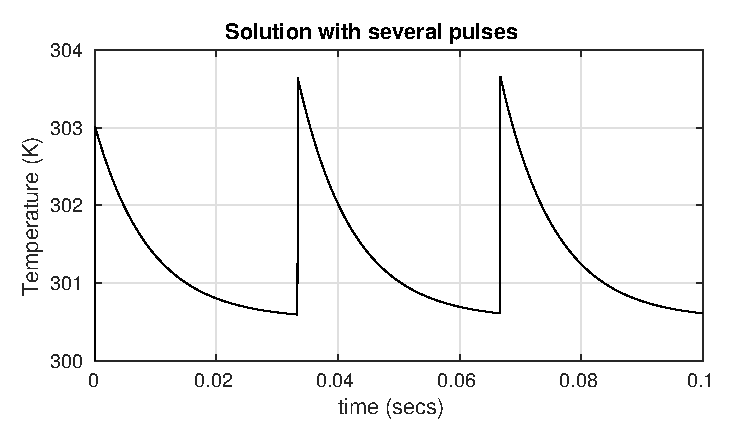
\includegraphics[scale=0.9]{gfx/fig1_several_pulses.eps}
\caption{Solution to the heat balance equation~\eqref{eq:heat_balance_equation}.} \label{fig:solution_heat_balance_eq}
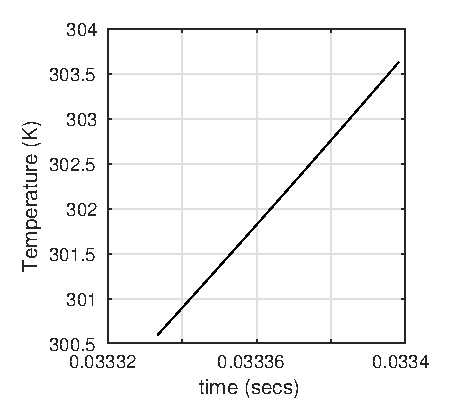
\includegraphics[scale=0.9]{gfx/fig1_int_time.eps}
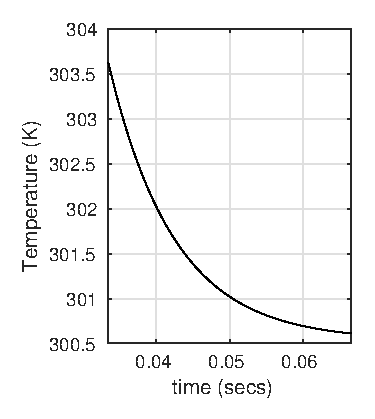
\includegraphics[scale=0.9]{gfx/fig1_cooling.eps}
\caption{Solution to the heat balance equation~\eqref{eq:heat_balance_equation} during the integration time $V_b>0$, and during the cooling time $V_b=0$. } \label{fig:solution_heat_balance_eq_splitted}
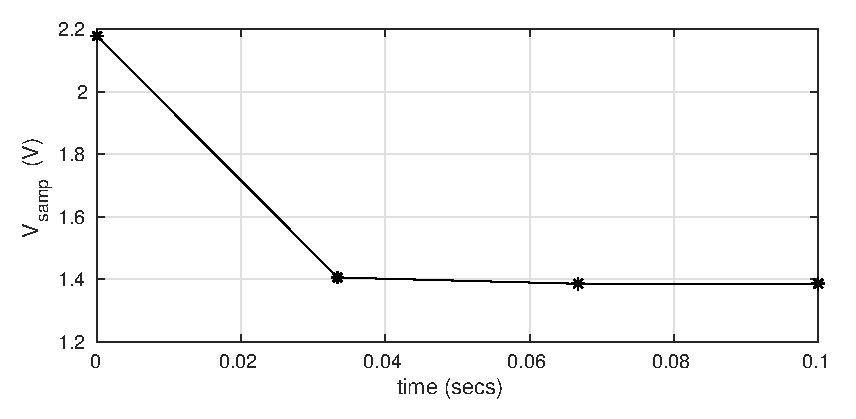
\includegraphics[scale=0.9]{gfx/fig1_Vout_several_pulses.eps}
\caption{Readout voltage~\eqref{eq:Vsamp_def}} \label{fig:Vout}
\label{fig:noisysol}
\end{figure}


As we can see in
Figure~\ref{fig:solution_heat_balance_eq}-\ref{fig:solution_heat_balance_eq_splitted},
the temperature of the bolometer does not only depend on the incoming
IR radiation, namely the temperature of the object we are observing,
but also on the bias voltage. In order to mitigate this phenomena, the
frame-time $t_f$ is set much larger than the integration time $t_i$ to
avoid overheat the bolometer. In particular the function temperature
$T$ oscillates in the time (after very few pulses) around the
temperature due to the incoming IR radiation. This also reflects in
the readout, since $V_{samp}$ becomes constant, i.e., the bolometer
has cached the temperature of the observed object.


\begin{center}
\begin{table}[]
\centering
\caption{Parameters and coefficients used in Section~\ref{sec:example}}
\label{tab:par_coeffs_example}
\begin{tabular}{|c|cr|c|cr|}
\hline
 $t_i$ 		& $65$ 		& $  \mu sec$ 		& $\alpha$  	&    	$-0.02$	&			\\
\hline
 $tf$ 		& $1/30$ 	& $  sec$ 	 	& $e$ 		&    	$0.8$ 	&			\\
\hline
 $R_S$ 		& $800 $ 	& $  k \Omega$ 		& $A$ 		&    	$17  $ 	& $ \mu m$ (square)	\\
\hline
 $T_s$		& $300 $ 	& $  K$ 	 	& $A_s$ 	&    	$17  $ 	& $ \mu m$ (square)	\\
\hline
 $G_{leg}$	&  $250 $ 	& $   \mu W K^{-1}$	& $\tilde C$ 	&	$4$ 	& $   p F$		\\
\hline
 $C$		&  $25 $ 	& $   n J K^{-1}$ 	& $V_0$		& 	$3.1$ 	& $   V$		\\
\hline
 $v_b$		& $3 $ 		& $   V$		& $E$		& 	$2$ 	& $   V$		\\
\hline
\end{tabular}
\end{table}
\end{center}

\subsection{Numerical methods for simulating the bolometer}
The output signal can be simulated by setting an initial temperature for the bolometer and by solving the heat balance equation~\eqref{eq:heat_balance_equation}. The readout $V_{samp}$ corresponds to the integral~\eqref{eq:Vsamp_def} that can be approximated with any numerical integration algorithm such as Riemann sum, trapezoidal rule, etc. The equation~\eqref{eq:heat_balance_equation} cannot be solved naively with a numerical scheme for ODE described, e.g., in \cite{mattheij1996ordinary,ascher1998computer}. Namely, any \texttt{matlab} ODE solver is not capable of solving~\eqref{eq:heat_balance_equation}. This is due to the fact that the function $V_b(t)$ (bias voltage), defined in~\eqref{eq:Vb}, has a very fast variation. The strategy for effectively solve the problem consists in splitting the domain in sub-domains where $V_b(t)$ is constant.

Assume that we want to solve~\eqref{eq:heat_balance_equation} for $0 \le t \le m t$ for a fixed $m \in \mathbb{N}$, namely we want $m$ pulses. The time domain can be split as
\begin{align*}
 [0, m t_f] = \bigcup_{k=0}^{m-1} (I_k \cup J_k)
\end{align*}
where $I_k=[k t, k t_f+t_i]$ and $J_k = [k t_f + t_i, (k+1)t_f]$.
We set $T_0(0):=T_0$ and for $k=1, 2, \dots$, we solve the ODE in $I_k$
\begin{align} \label{eq:heat_balance_equation_seq_bias}
& C\frac{dT_{k+1}}{dt}=\frac{v_b^2}{R(T_{k+1})}+\epsilon_e(P_t+P_s -2A\sigma T_{k+1}^4)-G_{leg}(T_{k+1}-T_s) \ , \ t \in I_k \nonumber \\
& T_{k+1}(kt_f)=T_{k}(kt_f)&
\end{align}
we set $\alpha:=T_{k+1}(kt_f+t_i)$ and we solve the ODE in $J_k$
\begin{align} \label{eq:heat_balance_equation_seq_no_bias}
& C\frac{dT_{k+1}}{dt}=\epsilon_e(P_t+P_s -2A\sigma T_{k+1}^4)-G_{leg}(T_{k+1}-T_s) \ , \ t \in J_k \nonumber \\
&T_{k+1}(kt_f+t_i)=\alpha_{k+1}
\end{align}
The solution $T(t)$ of~\eqref{eq:heat_balance_equation} is obtained by gluing the functions $T_j(t)$, i.e.,
\begin{align*}
 T(t) =
 \begin{cases}
  T_0(t) & t \in I_0 \cup J_0	\\
  T_1(t) & t \in I_1 \cup J_1	\\
	 & \vdots 		\\
  T_1(t) & t \in I_k \cup J_k	\\
	 & \vdots		\\
  T_m(t) & t \in I_m \cup J_m	\\
 \end{cases}
\end{align*}
In conclusion, the solutions of the ODEs~\eqref{eq:heat_balance_equation_seq_bias}-\eqref{eq:heat_balance_equation_seq_no_bias} can be approximated with any numerical scheme such us Euler method, Runge--Kutta, etc. We did not observe any difficulty in solving these equations and we chose the explicit Euler method as solver since this can easily be extended to the noised model (stochastic differential equation) that we will introduce in the next section.


%%% Local Variables:
%%% mode: latex
%%% TeX-master: "main"
%%% TeX-PDF-mode: 1
%%% TeX-PDF-via-dvips-ps2pdf: 1
%%% End:
